\chapter{The high-entropy silicide \ch{(CrFeMnNi)Si2}}
\label{sec:equi}

\section{$\beta$-\ch{FeSi2}}
We begin with a brief overview of the master compound $\beta-$\ch{FeSi2} that we have used as a foundation for the alloys in this project. In addition this is the sole case where our methods and results can be compared to experimental work and relevant literature.

$\beta$-\ch{FeSi_2} is a well known semiconductor with an experimentally measured band gap of around 0.85 eV at room temperature \cite{PhysRevB.58.10389}. The nature of the band gap is under debate, although most ab initio studies result in an indirect gap, experimental studies agree on a direct band gap. From our own calculations we get an indirect band gap of 0.65 eV with the PBE GGA functional. In comparison, Materials Project lists a band gap of 0.70 eV with the same functional. This slight discrepancy is most likely down to use of different parameters in the calculations, for instance Materials project use a different pseudopotential with more valence electrions, and a larger cutoff energy of 520 eV. In agreement with Materials Project our calculations return a final magnetic moment of the compound equal to 0. This can be seen in the electronic density of states plotted in figure 7.1, by that the DOS and hence band gap are identical in both spin directions.   

The formation energy $E_\text{form}$ of the compound can be calculated as the difference in total energy between the product and the sum of reactants. For the \ch{FeSi2} compound that consist of 16 iron atoms and 32 silicon we get 

\begin{equation*}
E_\text{form} = -327.72 \text{eV} - (16 \times -8.32 \text{eV} + 32 \times -5.42 \text{eV}) = -21.16 \text{eV}, 
\end{equation*}

or formation energy per atom $E_{FPA} = 0.441 eV$ from $-21.16/48$. The total energy of iron and silicon were calculated separately for the respective base elements with identical parameters as used for the \ch{FeSi2} calculation. The total energies correspond well with the listed energies from materials project of -8.4693 eV and -5.4234 eV for Fe, and Si respectively. Accordingly, the formation energy per atom for $\beta$-\ch{FeSi2} of 0.441 eV is in good agreement with materials project's value of 0.444 eV.

\begin{figure}[H]
\centering
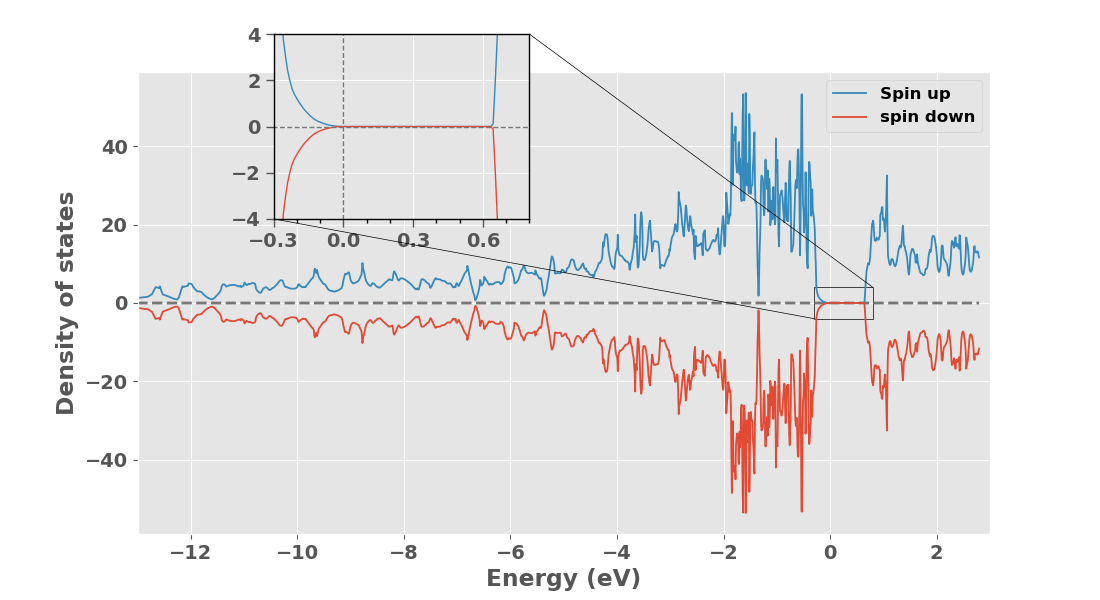
\includegraphics[width=\textwidth]{results/fesi2/bulk_DOS.png}
\caption{Density of states [states/eV] of $\beta$-\ch{FeSi2}}
\end{figure}
 

\section{\ch{(CrFeMnNi)Si2}}
The first alloy we will look at is the equimolar distribution of Cr, Fe, Mn and Ni. For details on this alloy, and a visualization of the supercells we refer the reader to section 6.2. Below in table 7.1 we list the total energy per atom, final magnetic moment per atom, and band gap of five distinct SQSs of the \ch{Cr4Fe4Mn4Ni4Si32} alloy. In addition we include the mean and standard deviation (std) between the 5 supercells and the formation energy calculated from the mean total energy. 
 
\begin{table}[H]
\centering
\begin{tabular}{@{}cccc@{}}
\toprule
SQS           & \begin{tabular}[c]{@{}c@{}}Toten \\ (eV)\end{tabular} & \begin{tabular}[c]{@{}c@{}}Mag \\ ($\mu_B$)\end{tabular} & \begin{tabular}[c]{@{}c@{}}$E_G$ \\ (eV)\end{tabular} \\ \midrule
A             & -6.608                                               & 0.083                                                   & 0.028                                                \\
B             & -6.614                                               & 0.083                                                   & 0.052                                                \\
C             & -6.606                                               & 0.083                                                   & 0.034                                                \\
D             & -6.616                                               & 0.083                                                   & 0                                                     \\
E             & -6.609                                               & 0.083                                                   & 0.050                                                \\ \midrule
Mean          & -6.611                                               & 0.083                                                   & 0.033                                                \\
Std           & 0.004                                                & 0.000                                                   & 0.021                                                \\
$E_{FPA} (eV)$   & -0.293                                          & -                                                        & -                                                     \\ \bottomrule
\end{tabular}
\caption{Total energy per atom (Toten), final magnetic moment per atom (Mag), band gap ($E_G$) and formation energy ($E_\text{FPA}$) of 5 SQS of \ch{(CrFeMnNi)Si2}.}
\end{table}

From table 7.1 we observe that the total energy and magnetic moment are quite similar in all 5 supercells, which could be expected from that the only variable between supercells is the atomic configuration. On the other hand, the atomic configuration has a larger impact on the band gap of the supercells. We find that the band gap ranges from a maximum value of 0.05 eV in SQS B, to a metal in SQS D, nevertheless much smaller than the band gap of 0.65 eV in \ch{FeSi2}. We will come back to the band gaps in section 7.2.1. 

Contrary to the master compound, these supercells representing the \ch{(CrFeMnNi)Si2} alloy contains a finite magnetic moment of around $0.083$  $\mu_B$. However, compared to a ferromagnet such as iron, with $\text{Mag} = 2.2$  $\mu_B$ according to Materials Project, we note that this is not a strong ferromagnetic material. In contrast to the high-entropy alloys discussed in section 2.2, we observe common for all supercells that the largest local magnetic moments are ascribed to chromium and manganese atoms in the lattice, while on the other hand both iron and nickel atoms within the numerical accuracy of the calculations, accounts for negligible contributions to the magnetic moment. Considering that the magnetic moment is identical across all five distinct atomic configurations, in addition to that the local magnetic moments displays very similar trends between supercells, the observed magnetism is probably connected to the specific crystal structure. It should be noted however that the magnetic properties in this project could be prone to errors. As we discussed in section 4.3, one of the major drawbacks of DFT in regards to magnetic materials is the local minima problem. In this project we have overlooked this concern, and applied a constant initial magnetic configuration to all structures, disregarding for example antiferromagnetic or possible permutations of ferrimagnetic orderings, to reduce the workload. Thus, its possible that the final magnetic structure of the supercells adopts local minima rather than global. Coupling this with the possible errors associated with the special quasi-random structures method to model the disordered magnetic structure means that the magnetic results and following the total energy and corresponding stability are not immutable nor necessarily accurate in respect to the hypothetical real alloy. 
    
In terms of the total energy the most and least stable SQSs are "D" and "A" respectively, meaning that SQS D is then the most representative configuration of the real material. However, most likely all five SQSs and other possible configurations would appear as local orderings in domains of the real material with a certain probability. Therefore we will consider and discuss the results of all 5 SQSs as well as the most stable supercell. Further, the total energy alone is not sufficient to evaluate the stability of the structure. In this project we have not considered factors such as the configurational entropy or made any finite temperature considerations. Additionally, the discussion above on the magnetic configuration could affect the total energy. Thus, the relative stability between supercells listed in table 7.1 could change. Nevertheless, we put the most effort into analyzing the most stable supercells of each alloy, as according to the considerations made in this project, are the most representative configurations of the real material.
\newpage
\subsection{The band gap}
As seen from table 7.1, the band gap of the alloy is severely reduced from the master compound, and varies between supercell to supercell. We observed a maximum band gap of 0.05 eV in SQS B, and on the flip side a 0 band gap in the most stable configuration, SQS D. The density of states of SQS D and B are displayed in figures 7.2 and 7.3 below. 

\begin{figure}[H]
	\centering
	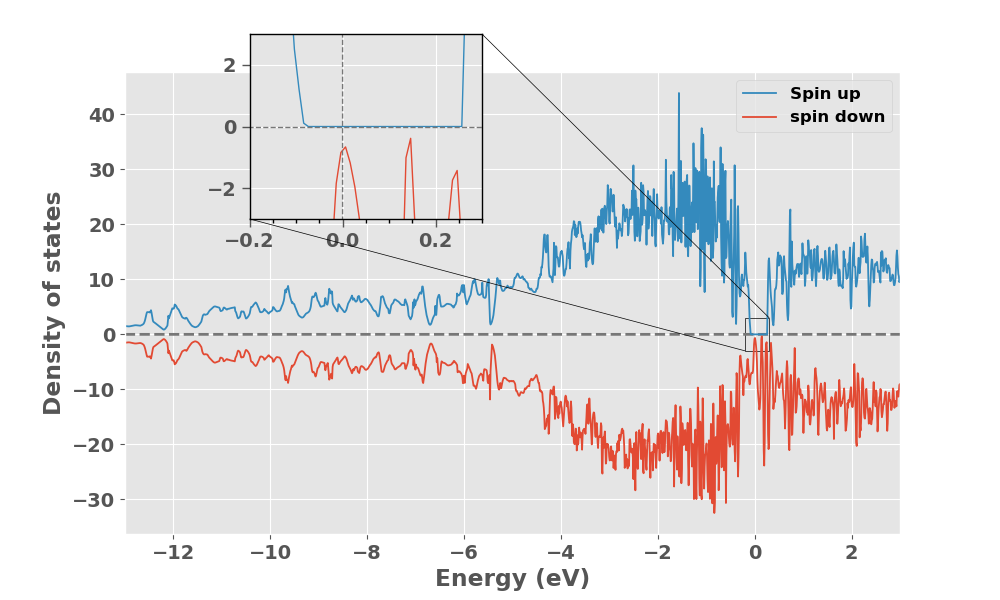
\includegraphics[width=\textwidth]{results/fesi2/D_TDOS.png}
	\caption{Density of states [states/eV] of SQS D of \ch{(CrFeMnNi)Si2}.}
\end{figure}

\begin{figure}[H]
\centering
	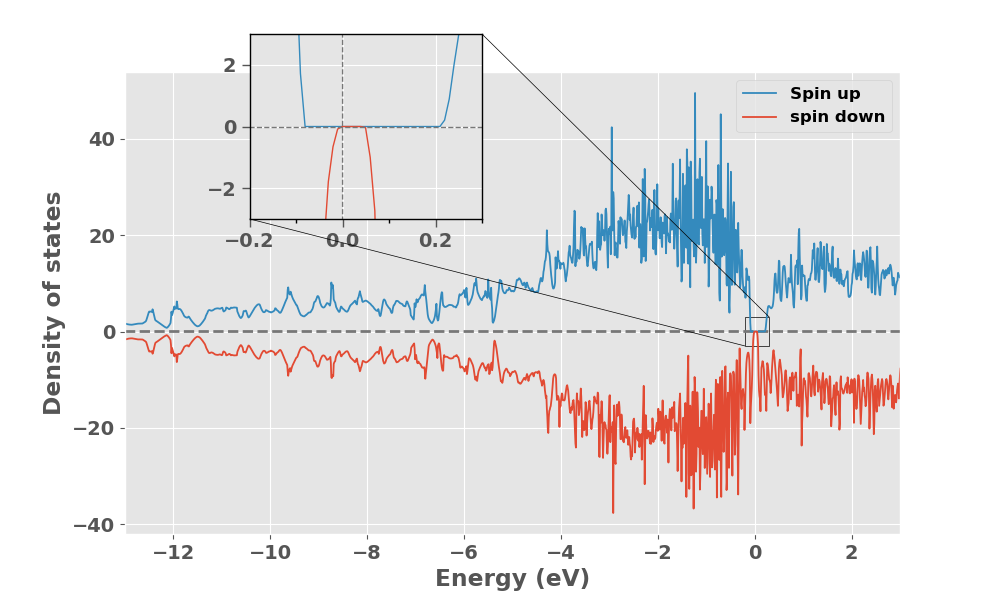
\includegraphics[width=\textwidth]{results/fesi2/B_TDOS.png}
	\caption{Density of states [states/eV] of SQS B of \ch{(CrFeMnNi)Si2}.}
\end{figure}  

In figure 7.2  and 7.3 we observe that the band gap in both SQS D and B, in accordance with the magnetic property differ between the spin directions. Going forward we will refer to the band gap in spin up as $E_G ^\text{up}$, and spin down as $E_G ^\text{dw}$. Clearly in both D and B $E_G ^\text{up} >> E_G ^\text{dw}$ as SQS D for instance exhibits a band gap of around 0.3 eV in spin up, contrary to a 0 in spin down. Comparing to the values in table 7.1 we find that the total band gaps of the respective structures are limited by the narrow or nonexistent band gap in spin down. 

To obtain further and more precise information on the band gap we look to the calculated Kohn-Sham eigenvalues. The band gaps found from investigating the eigenvalues, denoted as $E_G ^\text{eigen}$ can be seen below in table 7.2 for all five SQS. 

\begin{table}[H]
\centering
\begin{tabular}{@{}cccc@{}}
\toprule
SQS & \begin{tabular}[c]{@{}c@{}}$E_G ^\text{up, eigen}$ \\ (eV)\end{tabular} & \begin{tabular}[c]{@{}c@{}}$E_G ^\text{dw, eigen}$ \\ (eV)\end{tabular} & \begin{tabular}[c]{@{}c@{}}$E_G ^\text{tot, eigen}$ \\ (eV)\end{tabular} \\ \midrule
A   & 0.081                                                                     & 0.052                                                                     & 0.028                                                                    \\
B   & 0.293                                                                      & 0.052                                                                     & 0.052                                                                    \\
C   & 0.236                                                                      & 0.034                                                                     & 0.034                                                                    \\
D   & 0.340                                                                      & 0                                                                     & 0                                                                    \\
E   & 0.310                                                                      & 0.050                                                                     & 0.050                                                                    \\ \bottomrule
\end{tabular}
\caption{Band gap of five SQSs of \ch{(CrFeMnNi)Si2} in spin up, spin down and total. The band gaps are calculated from the Kohn-Sham eigenvalues of PBE simulations.}
\end{table}

Continuing the trend described above we observe equivalent to SQS D and B that $E_G ^\text{up} >> E_G ^\text{dw}$ for all supercells, par SQS A. In this supercell the spin polarization of the band gap is dampened, despite the supercell being equally magnetic to the other supercells. Moreover, in this case the total band gap $E_G ^\text{tot} =E_G ^\text{up} - E_G ^\text{dw}$, as opposed to the other supercells where the total band gap is equal to the lesser spin down band gap of the structure. This can be seen in the density of states in figure 7.4. DOS plots of SQS C and E can be seen in appendix A.1, note that in SQS C we were required to increase the number of points to calculate the density of states (NEDOS in VASP) in order to observe the band gap. 

\begin{figure}[H]
	\centering
	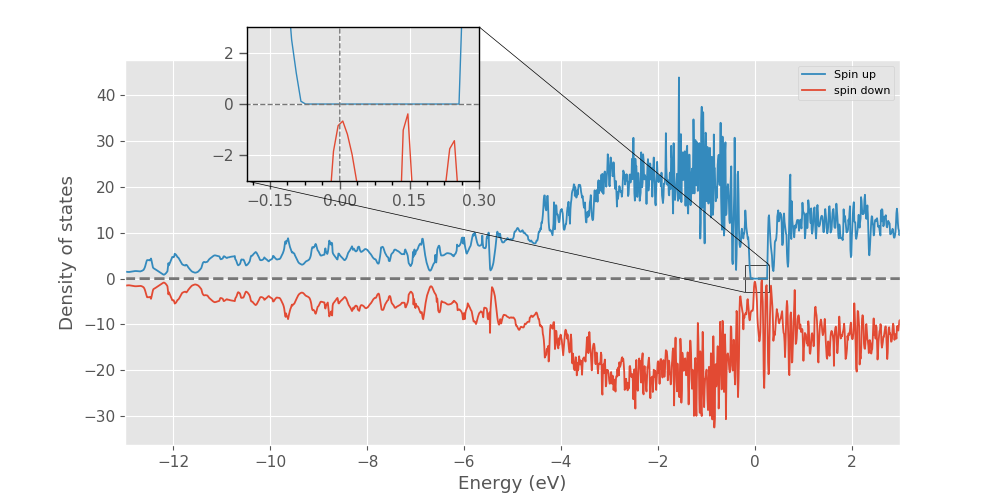
\includegraphics[width=.7\textwidth]{results/fesi2/A_TDOS.png}
	\caption{Density of states [states/eV] of SQS A of \ch{(CrFeMnNi)Si2}.}
\end{figure}


In VASP the energy eigenvalues are listed for every energy band at all k-points used in the calculation, with corresponding occupancy. An occupancy of 1 represents a fully occupied eigenstate, while a completely unoccupied (empty) eigenstate has occupancy equal to 0. We Recall that occupied states belong to the valence band, and the conduction band consists of unoccupied states (at 0 K). The highest energy valence band in these structures are band 124 in spin down and 128 in spin up, following the lowest energy valence band is 125/129 in spin down/up. The band gap in spin down is then determined from the difference between the lowest energy eigenvalue in band 125 and the highest energy eigenvalue in band 124, and likewise for the spin up band gap between bands 128 and 129. In SQS D different from the semiconducting structures we observe some partially occupied states at the band edges in bands 124 and 125 in spin down. With partially occupied states we refer to eigenstates in the valence band with occupancy less than 1 and states in the conduction band with occupancy above 0. Specifically, the highest energy eigenvalue (9.01 eV) in band 124 has occupancy equal to 0.94, and equivalently the lowest energy eigenvalue (8.98 eV) in band 125 has occupancy equal to 0.08. This results in a zero band gap. The Fermi energy of this structure is 8.99 eV, which means that the partially occupied eigenstate in band 124 is above the Fermi energy, and the partially unoccupied eigenstate in the conduction band below the Fermi energy. This is a clear indication of a metal, in which the conduction band and valence band overlap. In this project we will refer to such eigenstates with partial occupancy as defect states. The effect of the defect states on the band gap of SQS D can be seen in table 7.3. Here we calculate the band gap as a function of the defect states by an occupancy cutoff parameter $occ$, such that $E_G (0.99, 0.01)$ is the band gap when only including eigenvalues with occupancy above 0.99 in the valence band and below 0.01 in the conduction band. For simplicity we will write this parameter as a single value, where $occ = 0.01$ represents occupancy equal to 1 - 0.01 in the valence band and 0 + 0.01 in the conduction band.

\begin{table}[H]
\centering
\begin{tabular}{@{}cccc@{}}
\toprule
occ              & \begin{tabular}[c]{@{}c@{}}$E_G ^\text{up, eigen}$ \\ (eV)\end{tabular} & \begin{tabular}[c]{@{}c@{}}$E_G ^\text{dw, eigen}$ \\ (eV)\end{tabular} & \begin{tabular}[c]{@{}c@{}}$E_G ^\text{tot, eigen}$ \\ (eV)\end{tabular} \\ \midrule
0.5              & 0.340                                                                      & 0                                                                        & 0                                                                      \\
0.05             & 0.340                                                                      & 0.021                                                                     & 0.021                                                                    \\
0.01             & 0.340                                                                      & 0.050                                                                     & 0.050                                                                    \\
0.001            & 0.340                                                                      & 0.073                                                                     & 0.073                                                                    \\
\textless 0.0001 & 0.340                                                                      & 0.086                                                                     & 0.086                                                                    \\ \bottomrule
\end{tabular}
\caption{Band gap of SQS D of \ch{(CrFeMnNi)Si2} as a function of occupancy cutoff $occ$ in the eigenvalues.}
\end{table}

From table 7.3 we find clear evidence of the defect states prohibiting the band gap in spin down in SQS D, compared to the semiconducting supercells that contain only fully occupied and unoccupied eigenstates. To investigate this effect to greater extent we compare the eigenvalues of SQS D to a pure metal, such as iron. In this case the energy bands (both spins) around the Fermi energy (5.8 eV) are populated mostly by partially filled eigenstates. Inside a single energy band we observe instances of both more than half-filled states above $E_F$, and less than half-filled states above $E_F$, thus a clear overlap between the conduction and valence band. In contrast we find no instances of partial occupants in pure Si, as in the semiconducting SQSs. Therefore we can firmly state that the "defect states" are associated with a metallic character. Compared to the pure metal however, the amount and severity of the partial occupants are very dampened in SQS D. The concept of defect or impurity states in the band gap has been found as a common feature of the band structure of random alloys \cite{PhysRevLett.104.236403}, however we have reservations about if this is a physical result or related to numerical factors. In addition to partial occupants in Fe and SQS D we observe a plural of unphysical states where the occupancy exceeds 1 and 0. Recalling that the discontinues Fermi surface of metals poses several obstacles on DFT calculations with respect to the smearing and number of k-points. This result could then be imagined as a consequence of numerical methods. For instance in SQS B we conducted three separate electronic calculations, one with the tetrahedron method (value listed in tables) and two calculations with Gaussian smearing with smearing width 0.05 and 0.005 eV. With the Gaussian method and smearing width $\sigma = 0.05 eV$ we get $E_G ^\text{up, eigen} = 0.299 eV$ and $E_G ^\text{dw, eigen} = 0.050 eV$. Further calculations with the Gaussian method with smearing width of 0.005 eV results in $E_G ^\text{up, eigen} = 0.293 eV$ and $E_G ^\text{dw, eigen} 0.052 eV$. Compared to the values in table 7.3 with TBC, we observe that Gaussian (0.005 eV) and TBC are identical, while Gaussian (0.05 eV) show some deviation. Furthermore we find that the eigenvalues of Gaussian 0.05 eV contain defect states, and that the spin down band gap, as we experienced for SQS D, can be enlarged from $E_G ^\text{dw, eigen}(0.01) = 0.170 eV$. However, in this case we find no instances of non-naturalistic states as we described above for SQS D with TBC.
  
In conclusion, the defect states observed in SQS D appear to be related to a metallic structure, however from the discussion above we have seen that the results could be subject to numerical factors as well. It would have been instructive to visualize and analyze the eigenvalues by plotting the band structure. Unfortunately this is neither simple to perform or interpret for large supercells consisting of several elements and a large number of energy bands. One solution could be band-unfolding, but this did not work in conjunction with the implementation of the SQS method in this project. 

\subsection{Local and projected density of states}
In this section we will analyze the local and projected density of states of primarily SQS D (most stable). Below we include the local density of states of silicon in figure 7.5, and the respective LDOS plots of the various 3d elements of the compound in figure 7.6.  
  
\begin{figure}[H]
	\centering
	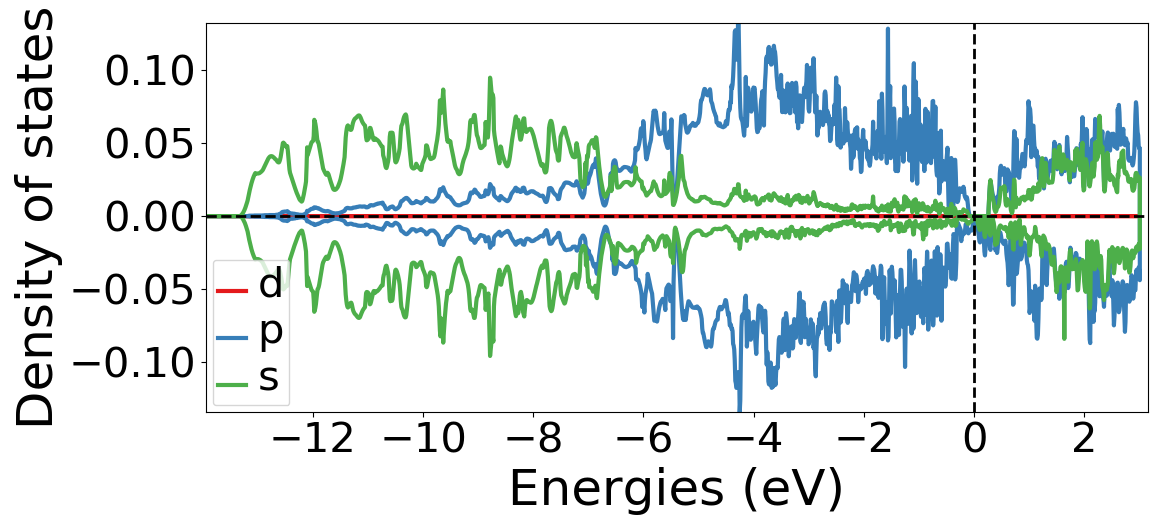
\includegraphics[width=.7\textwidth]{results/fesi2/D_LDOS_Si.png}
	\caption{Local density of states [states/eV] of Si, in SQS D of \ch{(CrFeMnNi)Si2}.}
\end{figure} 

\begin{figure}[H]
	\centering
	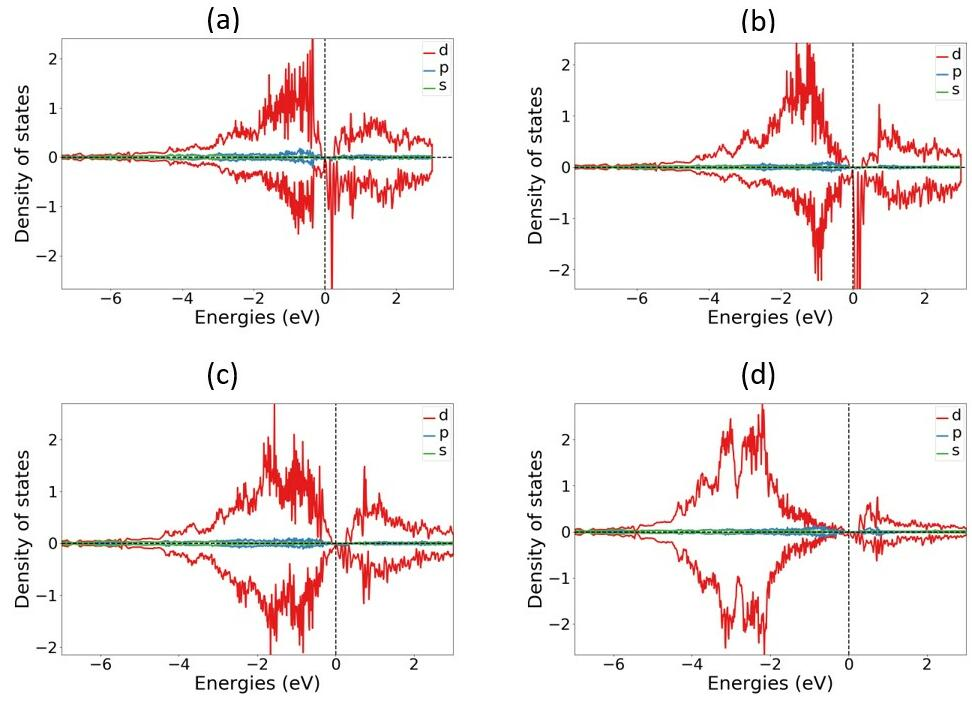
\includegraphics[width=\textwidth]{results/fesi2/D_LDOS.jpeg}
	\caption{Local density of states [states/eV] of (a) Cr, (b) Mn, (c) Fe, (d) Ni in SQS D of \ch{(CrFeMnNi)Si2}.}
\end{figure}   
  
In the local density of states of Si we see that the s-electrons in Si occupy states in the lower energy regions and p electrons at slightly elevated energies closer to the Fermi energy. Above $E_F$ states are occupied by s and p electrons equally. Between the 3d electrons of the transition metals, markedly manganese and chromium display a strong presence at energies just above $E_F$ and manganese additionally below $E_F$. Iron and Nickel show largest contributions at energies further from the Fermi energy, most notably bellow $E_F$. In the spin up channel we see a similar trend where chromium lie closest to $E_F$ followed by manganese, iron and lastly nickel at the lowest energies. The interplay between the 3d elements and silicon can be seen from the projected density of states in figure 7.7.

\begin{figure}[H]
	\centering
	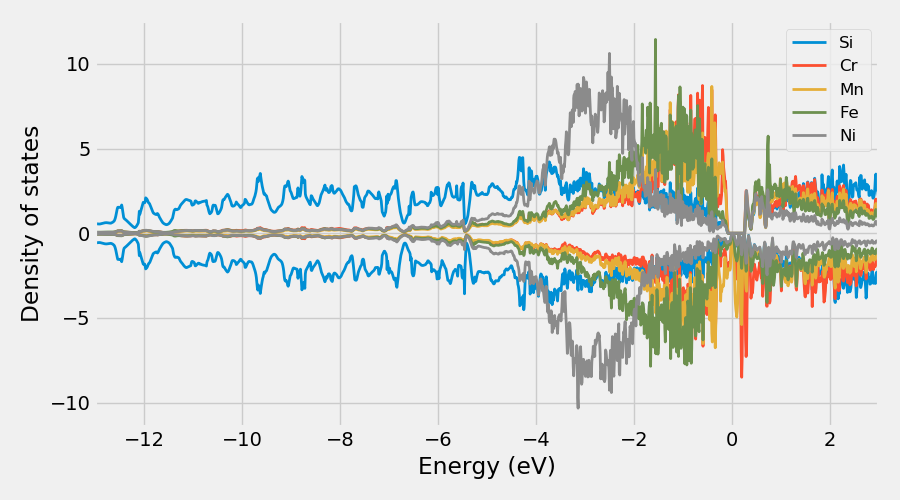
\includegraphics[width=.8\textwidth]{results/fesi2/D_PDOS.png}
	\caption{Projected density of states [states/eV] of SQS D of \ch{(CrFeMnNi)Si2}}
\end{figure} 

Compared to bulk $\beta$-\ch{FeSi2} \cite{doi:10.1063/1.346415}, we observe good agreement of the local DOS of Fe and Si in this alloy. Moreover the relative positions are in good agreement with observed trends in simpler Si-rich 3d transition metal silicides \cite{lange1997electronic}. In these compounds, the electronic structure tends to be dominated by d electrons, and the valence band density of states are filled by d states near $E_F$. The p-d hybridization between Si and TM elements is typically found at about 6 eV below $E_F$, and Si $s$ states about 10 eV below. In our alloy we observe good agreement of s-electrons as seen in the local density of states in figure 7.5, but the p electrons are pushed up in energy closer to $E_F$. 

\begin{figure}[H]
	\begin{subfigure}{.5\textwidth}
			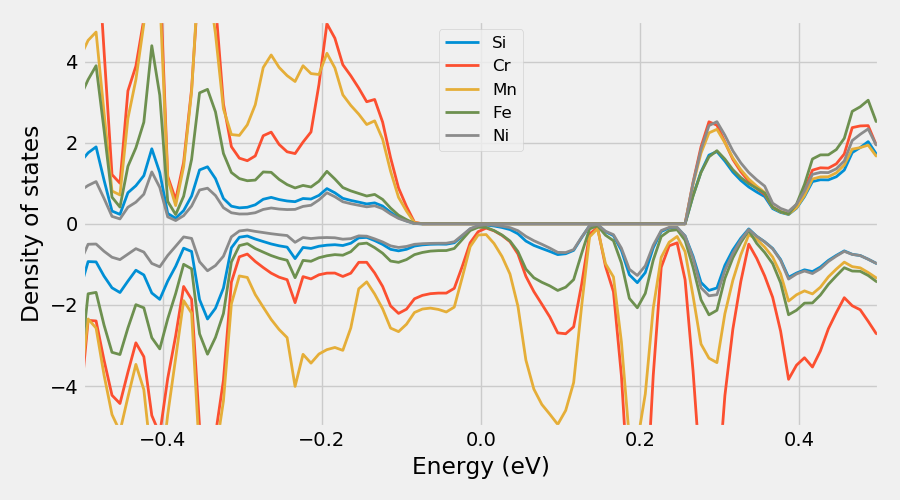
\includegraphics[width=\textwidth]{results/fesi2/D_PDOS_Ef.png}
			\caption{SQS D}		
	\end{subfigure}
	\begin{subfigure}{.5\textwidth}
		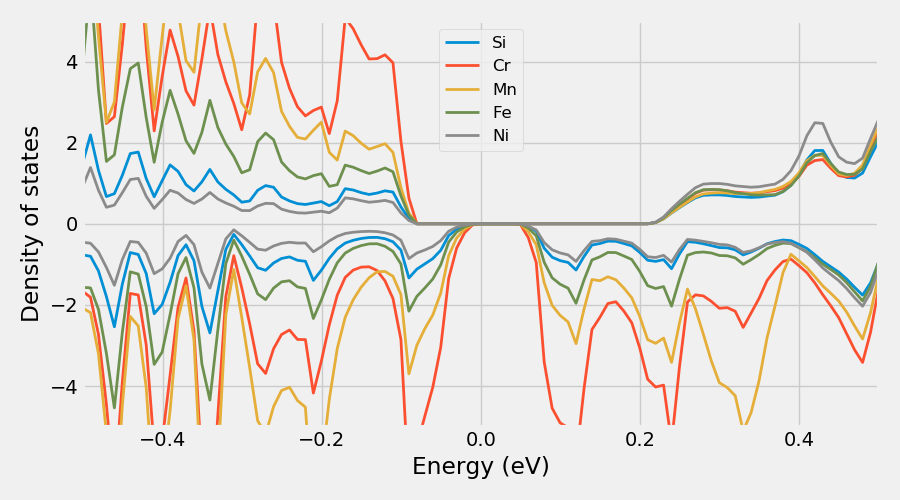
\includegraphics[width=\textwidth]{results/fesi2/B_PDOS_Ef.png}
		\caption{SQS B}		
	\end{subfigure}
	\caption{Projected density of states [states/eV] of SQS D and B of \ch{(CrFeMnNi)Si2} around the Fermi energy.}
\end{figure}

In figure 7.8 above we have plotted the projected DOS of the half-metallic structure (SQS D) and the configuration with the largest $E_G ^\text{dw}$) SQS B around the Fermi energy. Compared to the semiconducting structure we can distinctly observe a large number of Mn states in SQS D around $E_F$, most noticeably in spin down, but also in spin up. The projected density of states of SQSs A, B, and E are included in appendix A.2 (unable to plot PDOS for SQS C).

\subsection{The band gap of \ch{(CrFeMnNi)Si2} with SCAN and HSE06}
As expressed previously, in this work we invoke 3 steps of Jacob's ladder: GGA (PBE), meta-GGA (SCAN) and hybrid functional (HSE06), to determine the band gap. The outcome of these 3 functionals are showcased in table 7.4.

\begin{table}[H]
\centering
\begin{tabular}{@{}ccccc@{}}
\toprule
\multicolumn{1}{l}{SQS}                 & XC-functional & \begin{tabular}[c]{@{}c@{}}$E_G ^\text{up}$ \\ (eV)\end{tabular} & \begin{tabular}[c]{@{}c@{}}$E_G ^\text{dw}$ \\ (eV)\end{tabular} & \begin{tabular}[c]{@{}c@{}}$E_G ^\text{tot}$ \\ (eV)\end{tabular} \\ \midrule
\multicolumn{1}{c|}{\multirow{3}{*}{A}} & PBE           & 0.082                                                           & 0.052                                                           & 0.028                                                            \\
\multicolumn{1}{c|}{}                   & SCAN          & 0                                                                & 0                                                                & 0                                                                 \\
\multicolumn{1}{c|}{}                   & HSE06         & 0.708                                                           & 0.026                                                           & 0.026                                                            \\ \midrule
\multicolumn{1}{c|}{\multirow{3}{*}{B}} & PBE           & 0.293                                                           & 0.052                                                           & 0.052                                                            \\
\multicolumn{1}{c|}{}                   & SCAN          & 0.147                                                           & 0.089                                                           & 0.089                                                            \\
\multicolumn{1}{c|}{}                   & HSE06         & 0.286                                                           & 0.182                                                           & 0.182                                                            \\ \midrule
\multicolumn{1}{c|}{\multirow{3}{*}{C}} & PBE           & 0.236                                                           & 0.034                                                           & 0.034                                                            \\
\multicolumn{1}{c|}{}                   & SCAN          & 0.069                                                           & 0.112                                                           & 0.112                                                            \\
\multicolumn{1}{c|}{}                   & HSE06         & 0.174                                                           & 0.033                                                           & 0.020                                                            \\ \midrule
\multicolumn{1}{c|}{\multirow{3}{*}{D}} & PBE           & 0.339                                                           & 0                                                           & 0                                                                 \\
\multicolumn{1}{c|}{}                   & SCAN          & 0                                                                & 0.108                                                           & 0                                                                 \\
\multicolumn{1}{c|}{}                   & HSE06         & 0.378                                                           & 0                                                                & 0                                                                 \\ \midrule
\multicolumn{1}{c|}{\multirow{3}{*}{E}} & PBE           & 0.308                                                           & 0.050                                                           & 0.050                                                            \\
\multicolumn{1}{c|}{}                   & SCAN          & 0.154                                                           & 0.111                                                           & 0.105                                                            \\
\multicolumn{1}{c|}{}                   & HSE06         & 0.548                                                           & 0.013                                                           & 0.013                                                            \\ \bottomrule
\end{tabular}
\caption{Band gaps of five supercells of \ch{(CrFeMnNi)Si2} in spin up, spin down and total, calculated with PBE, SCAN and HSE06 functionals.}
\end{table}

We will begin dissecting table 7.4 by comparing SCAN to PBE. The first distinction we make notice of is in SQS A. Here calculations with the SCAN functional predicts a metallic compound, contrary to the the PBE band gap of 0.03 eV. Alike the band gap of SQS D discussed previously, the 0 band gap in this structure with SCAN is caused by defect states. Neglecting such states and evaluating the band gap from exclusively almost completely filled and empty eigenstates yield $E_\text{G, SCAN} ^{up, eigen}(0.01) = 0.032$ eV and $E_\text{G, SCAN} ^{dw, eigen}(0.01) = 0.053$ eV, and a total band gap of 0.032 eV. This value seems to agree better with the PBE band gap of this supercell, but we observe that $E_G ^\text{up}$ is larger in PBE.  This is a recurrent pattern with SCAN across all five SQSs, where $E_\text{G, SCAN} ^\text{up} < E_\text{G, PBE} ^\text{up}$, and moreover $E_\text{G, SCAN} ^\text{dw} > E_\text{G, PBE} ^\text{dw}$. This can be seen in figure 7.9, where we plot the density of states of SQS E (a, b) and C (c, d). Note that the SCAN band gap in SQS C has the opposite spin polarization of PBE; this is also the case in SQS D, as seen in table 7.4.
\begin{figure}[H]
	\begin{subfigure}{.5\textwidth}
		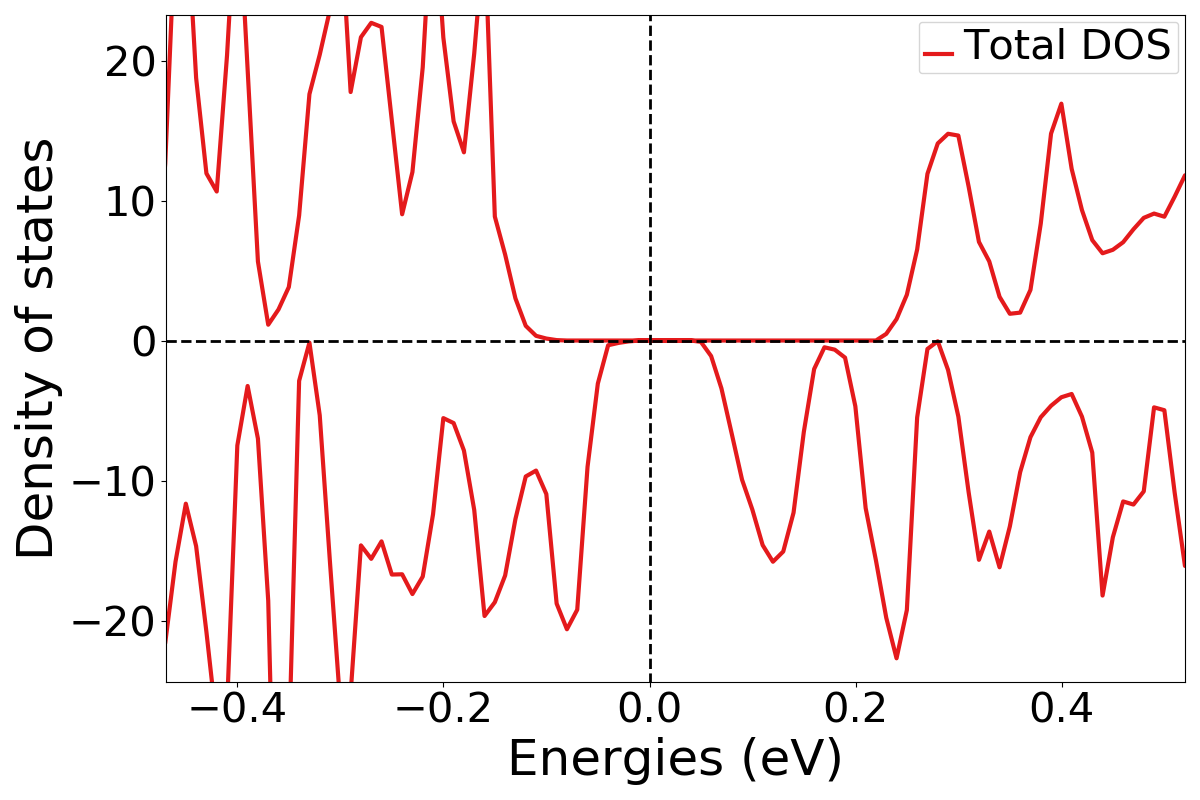
\includegraphics[width=\textwidth]{results/fesi2/E_DOS_pbe.png}
		\caption{SQS E PBE}
	\end{subfigure}
	\begin{subfigure}{.5\textwidth}
		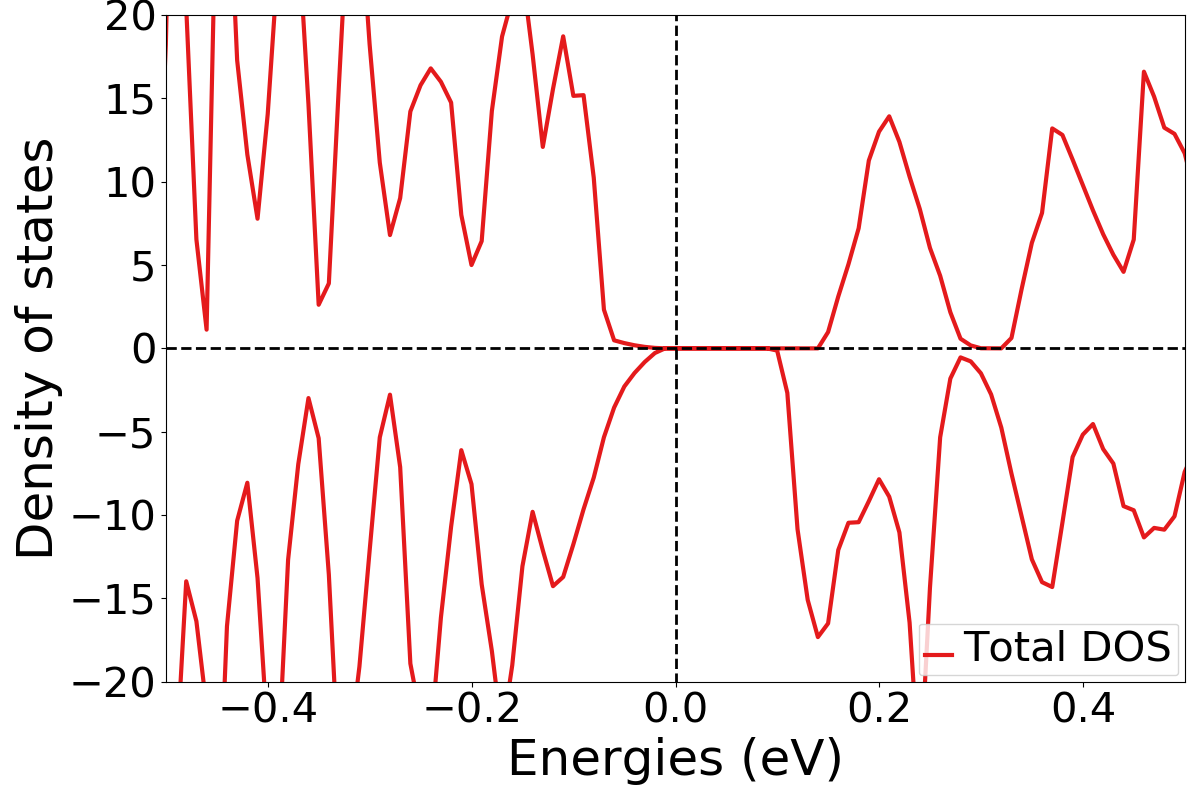
\includegraphics[width=\textwidth]{results/fesi2/E_DOS_scan.png}
		\caption{SQS E SCAN}
	\end{subfigure}
	\begin{subfigure}{.5\textwidth}
		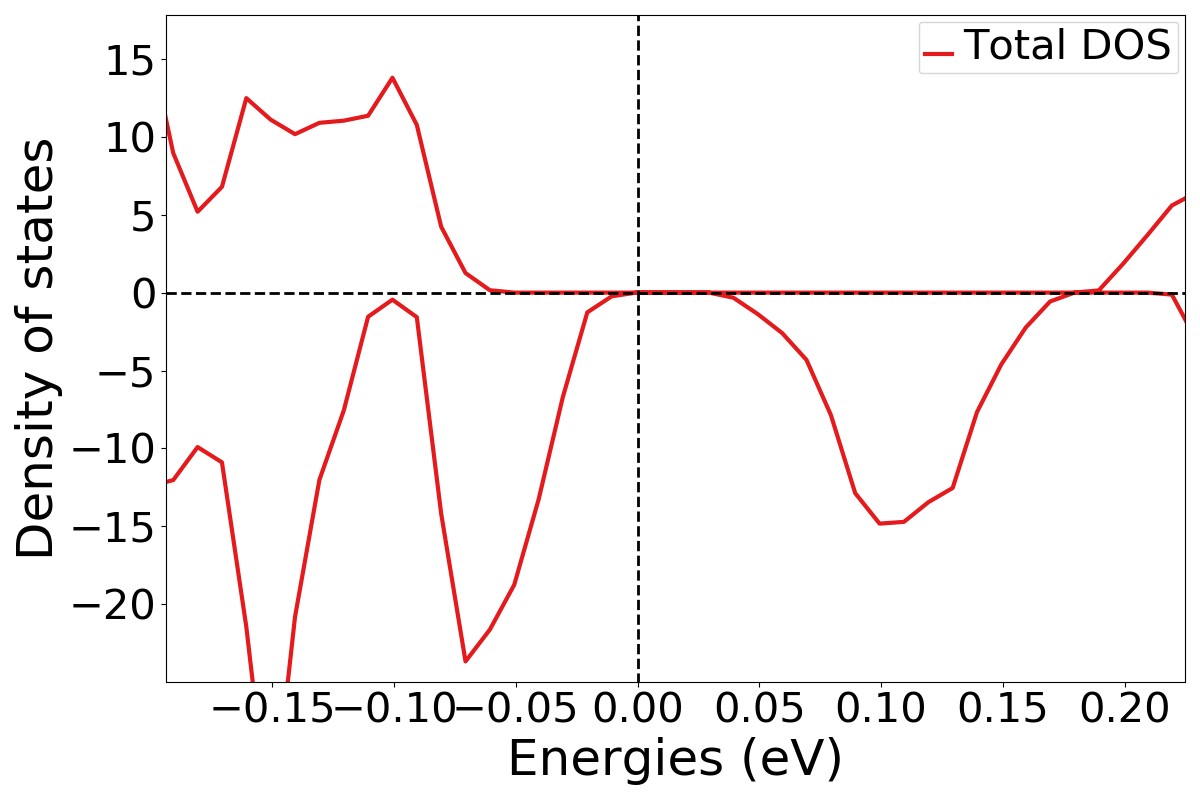
\includegraphics[width=\textwidth]{results/fesi2/C_DOS_pbe.png}
		\caption{SQS C PBE}
	\end{subfigure}
	\begin{subfigure}{.5\textwidth}
		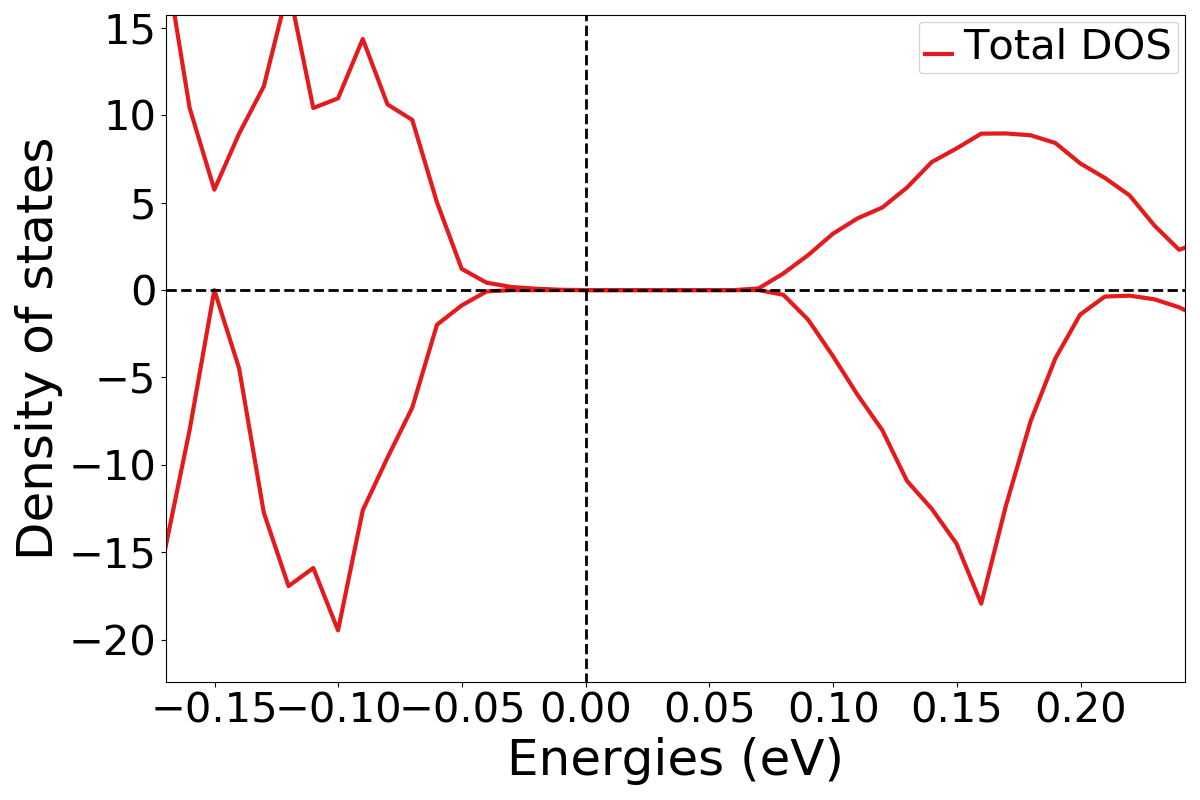
\includegraphics[width=\textwidth]{results/fesi2/C_DOS_scan.png}
		\caption{SQS C SCAN}
	\end{subfigure}
	\caption{Density of states [states/eV] illustrating the difference between band gaps of SQS E and D of \ch{(CrFeMnNi)Si2} with PBE and SCAN.}
\end{figure}

\begin{figure}[H]
	\centering	
	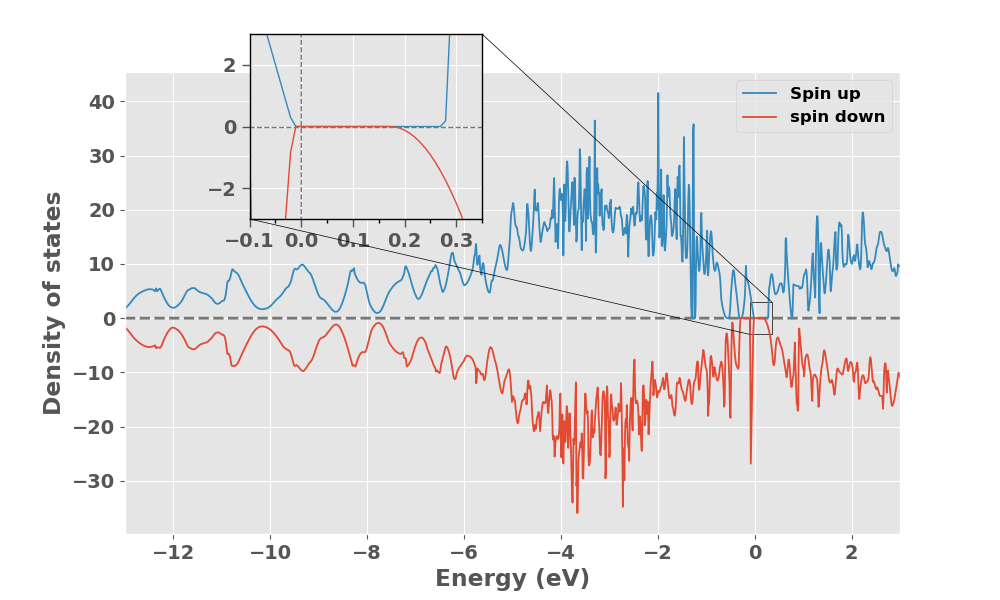
\includegraphics[width=.95\textwidth]{results/fesi2/B_TDOS_hse06.png}
	\caption{Density of states [states/eV] of SQS B of \ch{(CrFeMnNi)Si2} with HSE06.}
\end{figure}

With the HSE06 functional we observe the opposite trend in SQS A and E compared to SCAN, here $E_\text{G, HSE06} ^\text{up} > E_\text{G, PBE} ^\text{up}$ and $E_\text{G, HSE06} ^\text{dw} < E_\text{G, PBE} ^\text{dw}$. But in other cases $E_\text{G, HSE06} ^\text{up}$ is lesser (SQS C) or similar to PBE (SQS B and D). On the other hand $E_\text{G, HSE06} ^\text{dw}$ is consistently smaller in all structures compared to PBE, with the exception of SQS B. In this structure the HSE06 functional predicts large band gaps in both spin directions, this can be seen in the density of states plotted in figure 7.10 above.    
 
  
As we discussed in section 5.1, hybrid functionals are much more computationally demanding compared to both meta-GGA and GGA functionals. In this project we experienced particular difficulty of converging calculations with HSE06 of the compositionally complex SQSs. To reduce the cost of the HSE06 functional we performed such calculations with a lower density of k-points, see section 6.1. The small amount of k-points could as discussed lead to numerical inaccuracies relating to the calculation of the Fermi surface in metallic structures. Furthermore, the reduced mesh of k-points could result in artificially exaggerated band gaps from failing to encapsulate the exact minimum transition between the valence band and conduction band.

\begin{table}[H]
\centering
\begin{tabular}{@{}lc@{}}
\toprule
XC-functional & \begin{tabular}[c]{@{}c@{}}Transition \\ (k-point)\end{tabular} \\ \midrule
PBE           & (1/4, 0, 1/4) $\rightarrow$ (0, 0, 0)           \\
SCAN          & (1/4, 0, 1/4) $\rightarrow$ (0, 1/3, 0)           \\
HSE06         & (1/2, 0, 0) $\rightarrow$ (0, 0, 0)           \\ \bottomrule
\end{tabular}
\caption{Minimum gap between k-point in valence band and conduction band in SQS B of \ch{(CrFeMnNi)Si2} from PBE, SCAN and HSE06 simulations.}
\end{table}

In table 7.5 we list the transition between the highest occupied k-state in the valence band and lowest unoccupied k-state in the conduction band for SQS B with PBE, SCAN and HSE06 respectively. We  
observe that all 3 functionals find different k-point transitions. A concerning factor is that the highest energy k-point in the valence band from PBE calculations (1/4, 0, 1/4) is not included in the HSE06 calculation with the narrow mesh of 2x2x2 k-points. Thus, one may suspect that the HSE06 calculation overlooks the minimum transition and hence returns an enlarged band gap instead. This could be the case in $E_\text{G, A} ^{up}$ and $E_\text{G, B} ^{dw}$ where HSE06 predicts much larger values than PBE. However, without an experimental baseline we can not conclude that this is the case. As in the other instances we find that HSE06 produces similar or lower band gaps compared to PBE despite of the smaller number of k-points.     

As stated in section 6.2, we did not manage to converge the hybrid calculations using the tetrahedron method. We overcame this problem by first calculating the charge density using Gaussian smearing and utilizing the charge density to expedite TBC HSE06 calculations. The respective HSE06 band gaps of the five SQSs of of the \ch{(CrFeMnNi)Si2} system from utilizing both methods are displayed in table 7.6. Here, the band gap is calculated from the eigenvalues at different cutoff occupancy $occ$ to highlight the part of defect states.

\newpage
\begin{landscape}
\begin{table}[]
\vskip-1.5cm \hskip1cm \begin{tabular}{@{}cccccccc@{}}
\toprule
\multicolumn{1}{l}{SQS}                          & \begin{tabular}[c]{@{}c@{}}Smearing (type) \\ width (eV) \end{tabular} & \begin{tabular}[c]{@{}c@{}}$E_\text{G} ^{up, eigen}(0.5)$\\ (eV)\end{tabular} & \begin{tabular}[c]{@{}c@{}}$E_\text{G} ^{dw, eigen}(0.5)$\\ (eV)\end{tabular} & \begin{tabular}[c]{@{}c@{}}$E_\text{G} ^{up, eigen}(0.01)$\\ (eV)\end{tabular} & \begin{tabular}[c]{@{}c@{}}$E_\text{G} ^{dw, eigen}(0.01)$\\ (eV)\end{tabular} & \begin{tabular}[c]{@{}c@{}}$E_\text{G} ^{tot, eigen}(0.5)$\\ (eV)\end{tabular} & \begin{tabular}[c]{@{}c@{}}$E_\text{G} ^{tot, eigen}(0.01)$\\ (eV)\end{tabular} \\ \midrule
\multicolumn{1}{c|}{\multirow{3}{*}{A}}          & \begin{tabular}[c]{@{}c@{}}Gaussian \\ (0.05)\end{tabular}    & 0.784                                                                        & 0.149                                                                        & -                                                                              & 0.298                                                                         & 0.149                                                                         & 0.298                                                                                \\
\multicolumn{1}{c|}{}                            & \begin{tabular}[c]{@{}c@{}}Gaussian \\ (0.005)\end{tabular}   & 0.212                                                                        & 0.101                                                                        & -                                                                              & -                                                                              & 0.101                                                                         & -                                                                                     \\
\multicolumn{1}{c|}{}                            & TBC                                                           & 0.708                                                                        & 0.026                                                                        & -                                                                              & -                                                                              & 0.026                                                                         & -                                                                                     \\ \midrule
\multicolumn{1}{c|}{\multirow{3}{*}{B}}          & \begin{tabular}[c]{@{}c@{}}Gaussian \\ (0.05)\end{tabular}    & 0.278                                                                        & 0.170                                                                        & 0.299                                                                         & 0.314                                                                         & 0.151                                                                         & 0.298                                                                                \\
\multicolumn{1}{c|}{}                            & \begin{tabular}[c]{@{}c@{}}Gaussian \\ (0.005)\end{tabular}   & 0.284                                                                        & 0.182                                                                        & -                                                                              & -                                                                              & 0.180                                                                         & -                                                                                     \\
\multicolumn{1}{c|}{}                            & TBC                                                           & 0.286                                                                        & 0.182                                                                        & -                                                                              & -                                                                              & 0.181                                                                         & -                                                                                     \\ \midrule
\multicolumn{1}{c|}{\multirow{3}{*}{C}}          & \begin{tabular}[c]{@{}c@{}}Gaussian \\ (0.05)\end{tabular}    & 0.108                                                                        & 0.106                                                                        & 0.241                                                                         & 0.184                                                                         & 0.065                                                                         & 0.184                                                                                \\
\multicolumn{1}{c|}{}                            & \begin{tabular}[c]{@{}c@{}}Gaussian \\ (0.005)\end{tabular}   & 0.130                                                                        & 0.022                                                                        & -                                                                              & -                                                                              & 0.022                                                                         & -                                                                                     \\
\multicolumn{1}{c|}{}                            & TBC                                                           & 0.174                                                                        & 0.033                                                                        & -                                                                              & -                                                                              & 0.020                                                                         & -                                                                                     \\ \midrule
\multicolumn{1}{c|}{\multirow{3}{*}{\textbf{D}}} & \begin{tabular}[c]{@{}c@{}}Gaussian \\ (0.05)\end{tabular}    & 0.366                                                                        & 0.059                                                                        & -                                                                              & 0.187                                                                         & 0.059                                                                         & 0.187                                                                                \\
\multicolumn{1}{c|}{}                            & \begin{tabular}[c]{@{}c@{}}Gaussian \\ (0.005)\end{tabular}   & 0.374                                                                             & 0.072                                                                         & -                                                                             & -                                                                             & 0.072                                                                             & -                                                                                    \\
\multicolumn{1}{c|}{}                            & TBC                                                           & 0.378                                                                        & 0                                                                             & -                                                                              & 0.267                                                                         & 0                                                                              & 0.267                                                                                \\ \midrule
\multicolumn{1}{c|}{\multirow{3}{*}{E}}          & \begin{tabular}[c]{@{}c@{}}Gaussian \\ (0.05)\end{tabular}    & 0.665                                                                        & 0.144                                                                        & -                                                                              & 0.168                                                                         & 0.144                                                                         & 0.168                                                                                \\
\multicolumn{1}{c|}{}                            & \begin{tabular}[c]{@{}c@{}}Gaussian \\ (0.005)\end{tabular}   & 0.583                                                                        & 0.121                                                                        & -                                                                              & -                                                                              & 0.121                                                                         & -                                                                                     \\
\multicolumn{1}{c|}{}                            & TBC                                                           & 0.548                                                                        & 0.013                                                                        & -                                                                              & -                                                                              & 0.013                                                                         & -                                                                                     \\ \cmidrule(l){2-8} 
\end{tabular}
\caption{Band gap of five supercells of \ch{(CrFeMnNi)Si2} from HSE06 calculations using Gaussian smearing, with smearing width $\sigma$ equal to 0.05 eV and 0.005 eV, and the tetrahedron method (TBC). "-"  means that the band gap are unchanged between occ = 0.5 and occ = 0.01.}
\end{table}
\end{landscape}
\newpage

As we experienced for SQS B (PBE) in section 7.2.1, defect states are only a factor in the calculations using Gaussian smearing with $\sigma$ = 0.05 eV. These band gaps contain defect states, and can consequently be enlarged. By comparing $E_G ^\text{up}$ and $E_G ^\text{dw}$ at $occ = 0.5$ and $occ = 0.01$, the defects appear to have a lesser role in spin up, as par SQS C the band gap in spin up is either consistent or only marginally different between the defect band gap and the hypothetical defect less band gap. $E_G ^\text{dw}$ on the other hand, increases significantly by removing the defect states. The Gaussian smearing method is generally in better agreement with TBC at lower smearing width. But even in this case we observe several dissimilarities. In SQS A and E, $E_G ^\text{dw}$ is larger with the Gaussian method, additionally $E_G ^\text{up}$ is much lower in SQS A. Furthermore, while the HSE06 band gap in SQS D using TBC is in good agreement with PBE, where both results in a spin up half-metal. The HSE06 calculation of this SQS using Gaussian smearing, predicts a semiconductor with band gap equal to $0.07 eV$ with $\sigma = 0.005$ eV. In this project we have based our choice of numerical smearing on the advice on the VASP manual stating that for accurate total energies and density of states in semiconductors, one should opt for the tetrahedron method \cite{ismear}.  However, seeing as our system is comprised of metals in addition to Si, we include the results from utilizing Gaussian smearing. There are of course many more factors that affect the accuracy and reliability of both methods, but these are outside the scope of this project.

The fact that the majority of functionals and SQS agree on the presence of a band gap is in itself an overwhelmingly positive result, that allow us to state with high certainty that the potential high-entropy silicide \ch{(CrFeMnNi)Si2} is in fact a semiconductor, or possibly a half-metal based on the observed spin polarization and the most stable configuration. Regarding the 3 functionals applied in this project, we experience best cohesion between PBE and HSE06 that both agree on a spin up polarization of the band gap, while SCAN predicts more symmetric band gaps. This can also be seen from the magnetic moment, whereas PBE and HSE06 yields a final magnetic moment (per atom) of 0.083 $\mu_B$ across all SQSs, with SCAN this is reduced to half the amount. In the nonmagnetic $\beta$-\ch{FeSi2} structure we find better agreement between PBE and SCAN. Both correctly predicts that the material is nonmagnetic, however compared to the experimental value of about 0.85 eV and the PBE band gap of 0.65 eV, we get a smaller band gap of 0.61 eV with SCAN. Thus, the SCAN functional does not necessarily result in increased accuracy over PBE, even in the  simpler nonmagnetic structure. To conclude this section on the band gap of the \ch{(CrFeMnNi)Si2} alloy, when studying the band gap with DFT, particularly PBE is well known to underestimate the band gap of the real material as we experienced for \ch{FeSi2}. Therefore, a band gap found with PBE
indicates the existence of a band gap of at least the same size of the real material. In the following sections, we will heavily emphasize the PBE functional to determine the band gap from both the fast and reliable use in addition to the points mentioned above. Furthermore, from our experiences in this project in conjunction with the lack of support, the SCAN function looks to perform quite poorly with respect to band gaps. The HSE06 functional on the other hand, yielded much more reliable results, however since it was often to computationally expensive and troublesome to implement for the structures in this project, we apply this scarcely in proceeding sections. 
 
\subsection{Pair distribution functions}
The pair distribution functions of SQS D and B are included below in figure 7.11. We compare the PDFs of the most stable configuration (SQS D) with those of SQS B to investigate distinctions between the half-metallic structure and the most stable semiconducting configuration (SQS B). 
 
\begin{figure}[H]
	\centering
	\begin{subfigure}{\textwidth}
		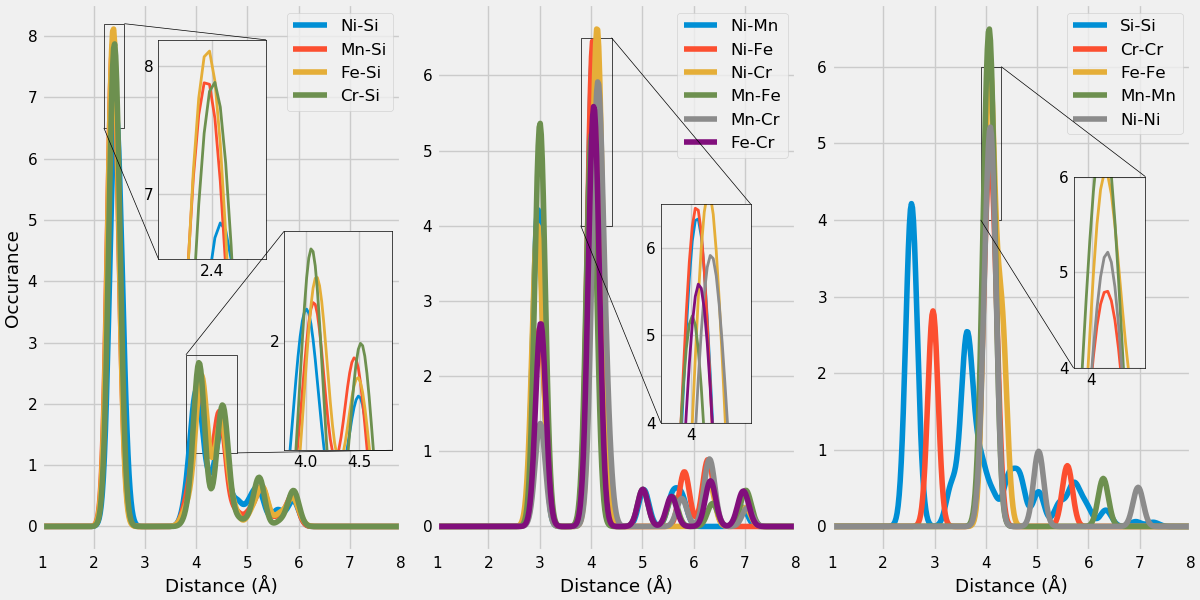
\includegraphics[width=\textwidth]{results/fesi2/D_PDF2.png}
	\end{subfigure}
	\begin{subfigure}{\textwidth}
		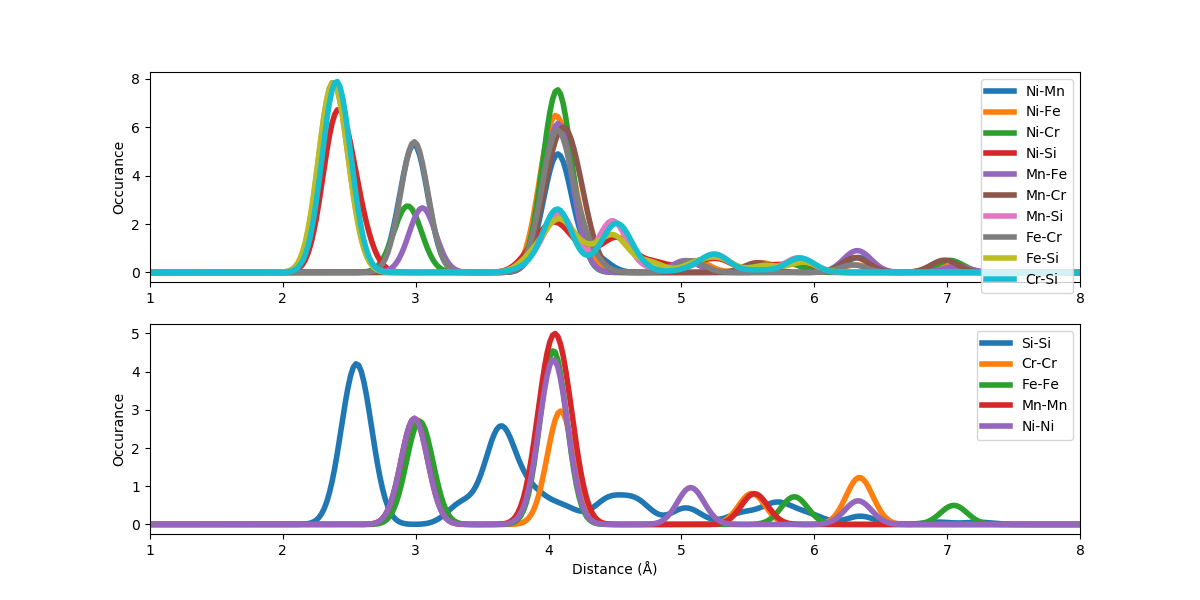
\includegraphics[width=\textwidth]{results/fesi2/B_PDF.png}
	\end{subfigure}
	\caption{Pair distribution functions of SQS D (top) and B (bottom) of \ch{(CrFeMnNi)Si2}.}
\end{figure}

With the aid of the ICSD \cite{icsd}, we can compare the PDFs in figure 7.11 to a compilation of PDFs based on a large number of experimental compounds. As these SQSs contains a total of 15 different bonds, comparing each one to the ICSD values would be an exhaustive process. According to the ICSD, the preferred bond-length of TM-Si bonds is observed at two values, with the shorter length the most occurring. Specifically Fe-Si bonds range between 2.25-2.75 Å and 4-5 Å, Mn-Si between 2.25-2.75 Å and 3.5-5 Å, Ni-Si between 2.25-2.5 Å and 3.85-5 Å, and finally Cr-Si between 2.35-2.65 Å and 4-5 Å. Clearly, the PDFs of the SQSs are in good agreement with the listed values of TM-Si bonds. The relative occurrence of the bonds between SQS D and B are mostly consistent, other than marginally reduced Fe-Si occurrence at 2.4 Å in B.

Nevertheless, we observe several differences between TM-TM bonds in SQS D and B, such as  Mn-Fe, Cr-Fe, and Ni-Mn bonds. This is simply a consequence of how the SQSs are generated; the silicon atoms are placed as before in the new supercells, but the TM elements are quasi-randomly distributed. Thus, it's reasonable that we would find the major differences between TM-TM bonds. Recalling that manganese in particular had a distinct presence in spin down around $E_F$ in SQS D, we observe that this particular supercell compared to SQS B has a preference of Mn-Fe bonds at 3 Å compared to Fe-Cr in SQS B, and overall larger preference of Mn-Mn bonds. However, the differences between PDFs are difficult to relate to the observed properties. Firstly because of the shear number of total bonds to analyze, and secondly considering the uniqueness of each SQS.

\subsection{Charge density}

Below we include the calculated charge density with PBE of SQS A, B, D and E of the \ch{(CrFeMnNi)Si2} alloy. We note that the half-metallic configuration (SQS D) appears to contain a marginally larger number of delocalized electronic charges in the lattice ,compared to the semiconducting SQSs. The charge density of SQS C is found in appendix A.3.

\begin{figure}[H]
\begin{subfigure}{.5\textwidth}
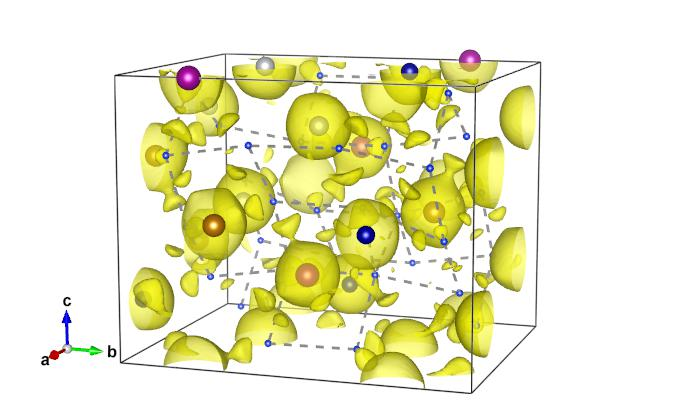
\includegraphics[width=\textwidth]{results/fesi2/A_CHGCAR.jpg}
\caption{SQS A}
\end{subfigure}
\begin{subfigure}{.5\textwidth}
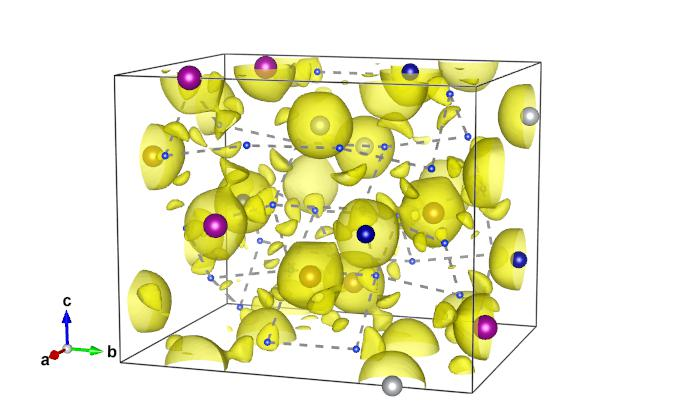
\includegraphics[width=\textwidth]{results/fesi2/B_CHGCAR.jpg}
\caption{SQS B}
\end{subfigure}
\begin{subfigure}{.5\textwidth}
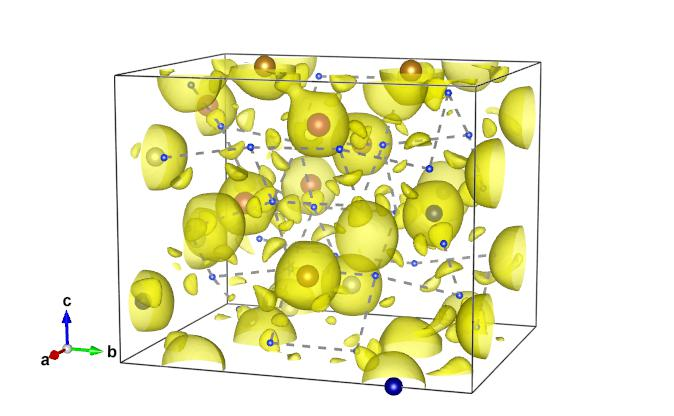
\includegraphics[width=\textwidth]{results/fesi2/D_CHGCAR.jpg}
\caption{SQS D}
\end{subfigure}
\begin{subfigure}{.5\textwidth}
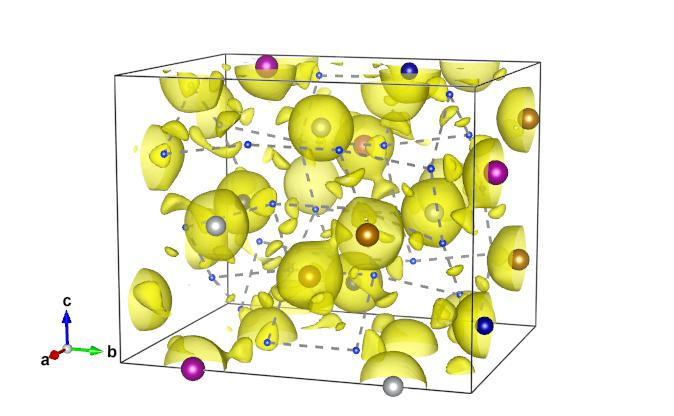
\includegraphics[width=\textwidth]{results/fesi2/E_CHGCAR.jpg}
\caption{SQS E}
\end{subfigure}
\caption{Contour plots of the Charge density of SQS A, B, D and E of \ch{(CrFeMnNi)Si2}.}
\end{figure}


\newpage
\subsection{SQS size}
Above we have presented the results of a high-entropy silicide \ch{(CrFeMnNi)Si2}, investigated by five 48-atom SQSs with a volume of 700 $\AA ^3$. This intermediate size allowed for more computationally affordable computations, and enabled us to calculate the band gap by more complex and expensive functionals, moreover test different settings, computational factors and compositions. However, as we discussed in section 4.3, the application of the SQS method to HEAs is not necessarily straightforward  The most pressing concern is the size of the SQS model and if it's sufficient enough to correctly model the disordered multi-component structure. In this section we will investigate factors of the SQS-method on the band gap and related results, by studying the difference between the 48 atom SQSs discussed above, to that of 96 and 192-atom SQSs with volumes 1200 $\AA ^3$ and 2400 $\AA ^3$ respectively. The computational cost of the 3 models are displayed below in figure 7.13 in terms of the number of CPU hours for both geometric and electronic relaxation of the structures.

\begin{figure}[H]
\centering
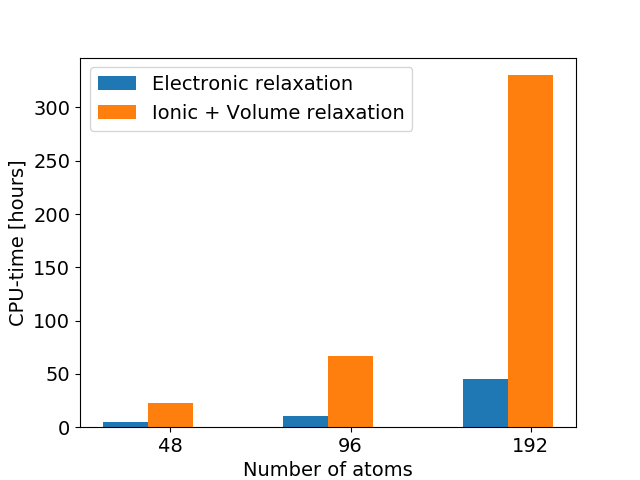
\includegraphics[width=.7\textwidth]{results/SQS_time.png}
\caption{CPU time of 48, 96 and 192-atom SQSs of \ch{(CrFeMnNi)Si2}}
\end{figure}

like the 48-atom model, the 96 and 192-atom SQS were tested by five unique configurations. In table 7.7 we list the mean and standard deviation from the set of configurations for all three sizes, with respect to the total energy per atom and final magnetic moment per atom, in addition to the formation energy of the mean total energy. Clearly, the 3 properties show minimal variation between the three sizes, furthermore we do not observe any indication of convergence with respect to the size. Thus, we may state that the 48-atom SQSs is sufficient for these materials. On the other hand, we observe that the larger models contain larger deviation between configurations, this can be expected given the increased total number of atoms that can vary between configurations. 

\begin{table}[H]
\centering
\begin{tabular}{@{}cccccc@{}}
\toprule
SQS size  & \multicolumn{2}{c}{\begin{tabular}[c]{@{}c@{}}Toten\\ (eV)\end{tabular}} & \multicolumn{2}{c}{\begin{tabular}[c]{@{}c@{}}Mag\\ ($\mu_B$)\end{tabular}} & \begin{tabular}[c]{@{}c@{}}$E_{FPA}$\\ (eV)\end{tabular} \\ \midrule
          & mean                                 & std                               & mean                                 & std                                  & mean                                                      \\ \midrule
48 atoms  & - 6.611                             & 0.004                                & 0.083                               & 0.000                               & -0.292                                                  \\
96 atoms  & - 6.609                             & 0.002                            & 0.071                               & 0.011                               & -0.292                                                 \\
192 atoms & - 6.612                             & 0.002                            & 0.076                               & 0.017                               & -0.295                                                 \\ \bottomrule
\end{tabular}
\caption{Total energy (Toten), magnetic moment (Mag) and formation energy ($E_text{FPA}$) of 48, 96 and 192 atom SQSs of \ch{(CrFeMnNi)Si2}}
\end{table}

The band gap corresponding to SQSs of each size are listed in table 7.8. First and foremost the band gap is evident in all three and exhibits analogous spin polarization, however appears to be less frequent and smaller in the larger structures. This result could simply be related to the uniqueness of each SQS, as also in the larger SQSs we observe sizable band gaps in certain configuration. Additionally, the larger cells has an increased possibility to create defect states.  

\begin{table}[H]
\centering
\begin{tabular}{@{}ccccc@{}}
\toprule
SQS size                                   & SQS        & \begin{tabular}[c]{@{}c@{}}$E_\text{G} ^{up, eigen}(0.5)$ \\ (eV)\end{tabular} & \begin{tabular}[c]{@{}c@{}}$E_\text{G} ^{dw, eigen}(0.5)$ \\ (eV)\end{tabular} & \begin{tabular}[c]{@{}c@{}}$E_\text{G} ^{tot, eigen}(0.5)$\\  (eV)\end{tabular} \\ \midrule
\multicolumn{1}{c|}{\multirow{5}{*}{48 atoms}}  & A          & 0.082                                                                         & 0.052                                                                         & 0.028                                                                          \\
\multicolumn{1}{c|}{}                     & B          & 0.293                                                                         & 0.052                                                                         & 0.052                                                                          \\
\multicolumn{1}{c|}{}                     & C          & 0.236                                                                         & 0.034                                                                         & 0.034                                                                          \\
\multicolumn{1}{c|}{}                     & \textbf{D} & 0.339                                                                         & 0                                                                              & 0                                                                               \\
\multicolumn{1}{c|}{}                     & E          & 0.308                                                                         & 0.050                                                                         & 0.050                                                                          \\ \midrule
\multicolumn{1}{c|}{\multirow{5}{*}{96 atoms}}  & \textbf{A} & 0.171                                                                         & 0.044                                                                         & 0.037                                                                          \\
\multicolumn{1}{c|}{}                     & B          & 0.139                                                                         & 0.027                                                                         & 0.027                                                                          \\
\multicolumn{1}{c|}{}                     & C          & 0.135                                                                         & 0.036                                                                         & 0.008                                                                          \\
\multicolumn{1}{c|}{}                     & D          & 0.089                                                                         & 0.040                                                                         & 0.040                                                                          \\
\multicolumn{1}{c|}{}                     & E          & 0.161                                                                         & 0                                                                              & 0                                                                               \\ \midrule
\multicolumn{1}{c|}{\multirow{5}{*}{192 atoms}} & A          & 0.120                                                                         & 0.032                                                                         & 0.032                                                                          \\
\multicolumn{1}{c|}{}                     & B          & 0.144                                                                         & 0                                                                              & 0                                                                               \\
\multicolumn{1}{c|}{}                     & C          & 0.187                                                                         & 0                                                                              & 0                                                                               \\
\multicolumn{1}{c|}{}                     & D          & \textit{0.048}                                                                & \textit{0.034}                                                                         & 0                                                                              \\
\multicolumn{1}{c|}{}                     & \textbf{E} & \textit{0.013}                                                                & \textit{0.018}                                                                         & \textit{0.013}                                                                          \\ \bottomrule 
\end{tabular}
\caption{Band gap of SQSs of 48, 96 and 192-atoms of \ch{(CrFeMnNi)Si2}. The names are arbitrary, A in 48 does not equal A in 96 or A in 192. The values listed in $italic$ relate to a defect band gap. Structures listed in bold text represents the most stable supercell of the set of SQSs.}
\end{table}

Equivalent to structure D in the 48 atom SQS, we find that the 0 band gap in SQS E in the 96 atom model suffers from defect states, without defects we find $E_\text{G} ^{dw, eigen}(0.01) = 0.016$ eV. The same is true for SQS B and C (192), but require $occ = 0.001$ to yield a small finite value. The band gap in SQS D and E (192) on the other hand, is finite at $occ = 0.5$, but can be enlarged from increasing $occ$, as we described for calculations utilizing Gaussian smearing with $\sigma$ = 0.05 eV. Specially, In SQS D (192-atoms), $E_\text{G} ^{up, eigen}(0.01) = 0.075$ eV and $E_\text{G} ^{dw, eigen}(0.01) = 0.05$ eV, similarly $E_\text{G} ^{up, eigen}(0.01) = 0.05$ eV, and $E_\text{G} ^{dw, eigen}(0.01) = 0.048$ eV in SQS E (192-atoms). In such cases where the eigenvalues inclusive of defect states return a finite band gap, the density of states does not. This is seen in figure 7.14 for SQS E in the 192-atom model that clearly has nonzero DOS at $E_F$ in both spin direction. 

\begin{figure}[H]
\centering
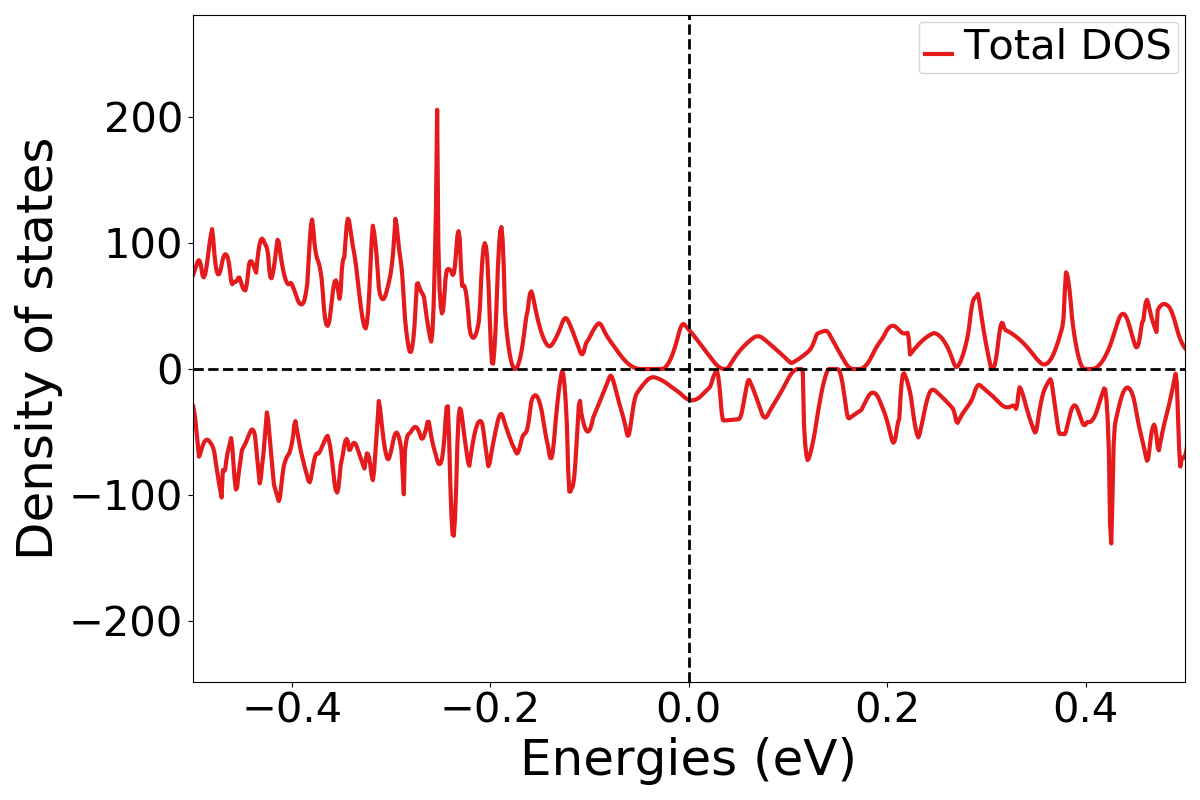
\includegraphics[width=.8\textwidth]{results/fesi2/192_E_DOS.png}
\caption{Density of states [states/eV] of SQS E of the 192-atom model of \ch{(CrFeMnNi)Si2}.}
\end{figure}    
 
One could wonder if the very narrow band gap in SQS E (192) of $0.013$ eV is subject to numerical precision in the DOS. But on the grounds of the small value we calculated the DOS in this case by 20000 points over the energy range -12 eV to 12 eV, which results in a resolution of about 8 points per 0.01 eV. In other words this should not be a factor. 
 
Drawing any conclusion on the band gaps is difficult seeing as we find very different results within all 3 sizes. The most stable SQSs suggests that the band gap converge towards a small or possible non-existent band gap with increasing SQS size. On the other hand we also find evidence of large band gaps in the larger cells in less stable configurations. This goes back to section 3.3 where we mentioned that one particular difficulty of the SQS method is the large number of possible atomic configurations of one compositions.    

Looking at the pair distribution functions of the most stable SQS in each model (figure 7.15), we observe that short-range interactions is well represented and identical across all three models. The distinctions between preferences as discussed in section 7.2.4 are most likely a product of the uniqueness of the SQSs more so than the size. On the other hand, the larger SQSs clearly provide a better description of long-range interactions that is not nearly as present in the smaller supercell. But, as seen from the minimal variation of the values in table 7.7 between the 3 models, in accordance with the fundamental philosophy of the SQS method, the functional properties are determined primarily from short-range interactions in the lattice. Thus, despite the fact that the larger SQSs offer improvements over the smaller SQSs, the gain is not justified by the increased computational cost.

\begin{figure}[H]
\begin{subfigure}{\textwidth}
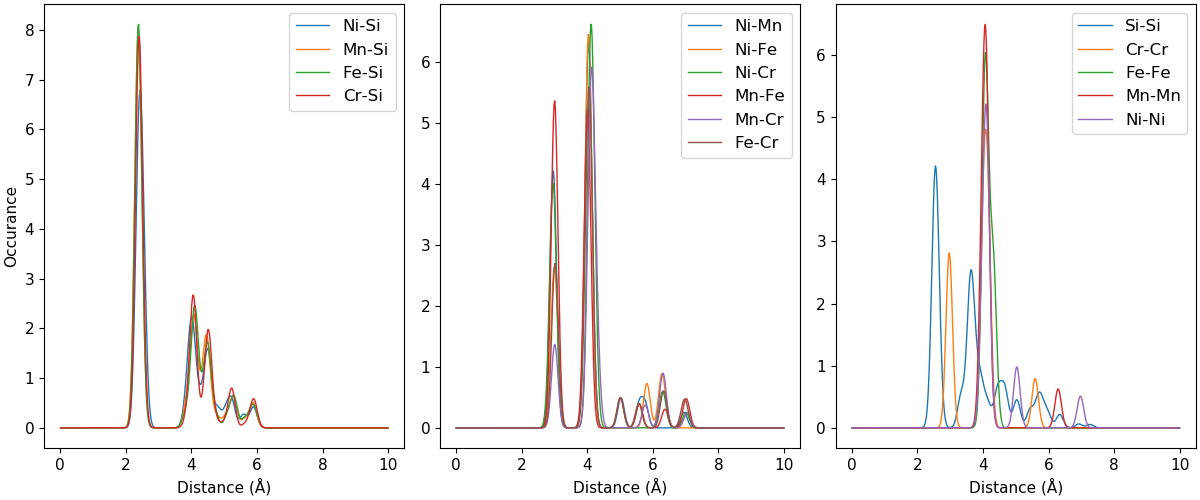
\includegraphics[width=\textwidth]{results/PDF48.png}
\end{subfigure}
\begin{subfigure}{\textwidth}
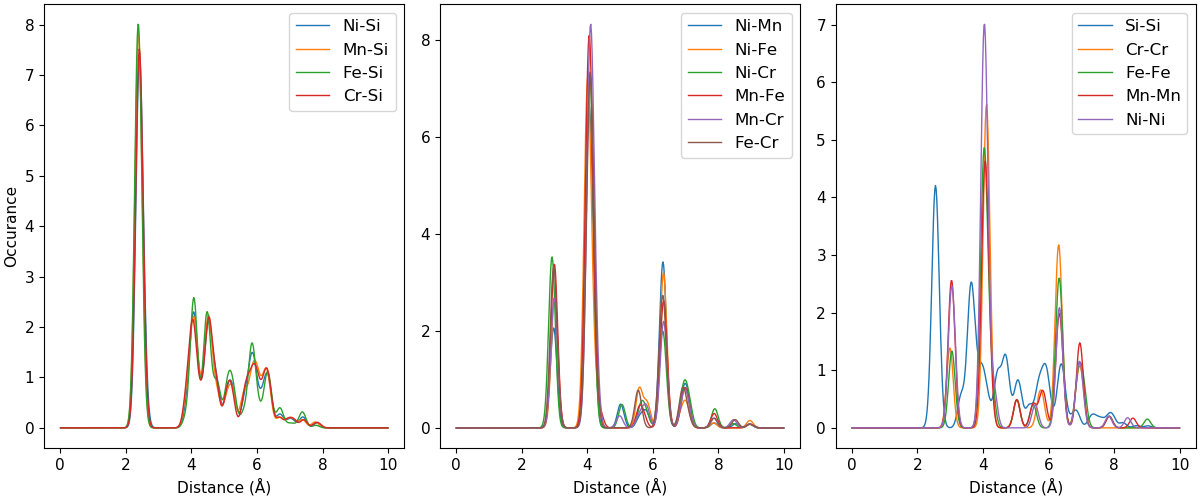
\includegraphics[width=\textwidth]{results/PDF96.png}
\end{subfigure}
\begin{subfigure}{\textwidth}
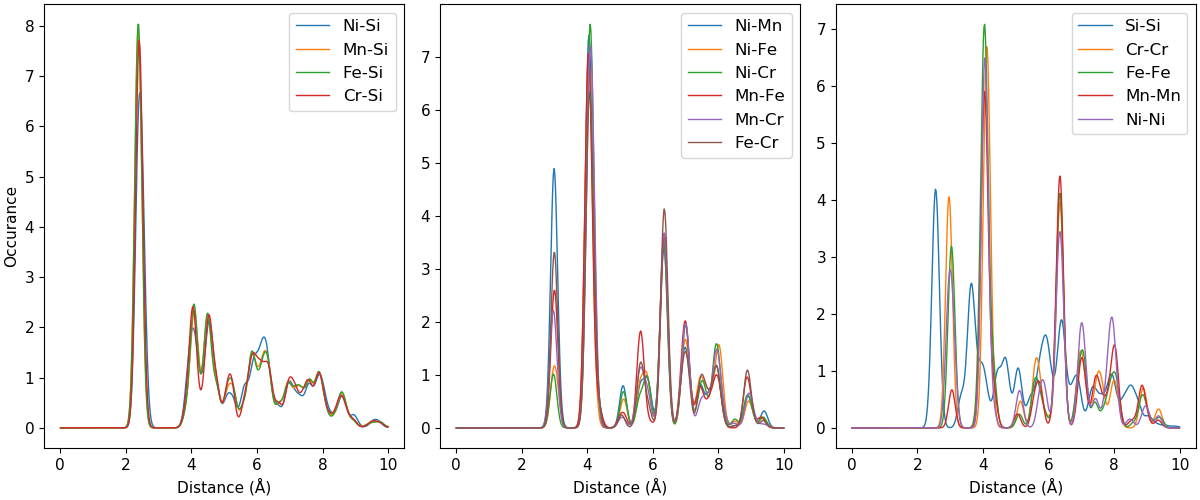
\includegraphics[width=\textwidth]{results/PDF192.png}
\end{subfigure}
\caption{Pair distribution functions of \ch{(CrFeMnNi)Si2} (top) 48-atom SQS, (middle) 96-atom SQS, (bottom) 192-atom SQS.}
\end{figure}
